\documentclass[12pt]{report}
\usepackage[english]{babel}
\usepackage[utf8]{inputenc}
\usepackage[hyphens]{url}
\usepackage{titlesec, float, graphicx}
\usepackage{enumitem}
\usepackage{graphicx}
\usepackage{listings}
\usepackage{amsmath}
\usepackage{xcolor}
\usepackage{courier}
\usepackage{amsmath}
\usepackage[final]{pdfpages}
\usepackage{caption}
\usepackage{subcaption} 
\usepackage{pdfpages}
\usepackage[unicode]{hyperref}

\newcommand\tab[1][1cm]{\hspace*{#1}}
\titleformat{\chapter}{\normalfont\huge}{\thechapter.}{20pt}{\huge}
\lstset{
	language=Java, 
	frame=single,
    breaklines=true,
    basicstyle=\ttfamily
    % postbreak=\mbox{\textcolor{red}{$\hookrightarrow$}\space}
    }
\begin{document}
%
% Zacatek titulni strany
%
\pagenumbering{gobble} 
\begin{center}

\includegraphics[scale=0.2]{img/ulpgc_logo.jpg}
\vspace{5cm}\linebreak
\Huge{Design of user interfaces}\linebreak
\large{Currency converter}\linebreak
\normalsize{2018/19 course - Practice 1}\linebreak
\vspace{3cm}\linebreak

\small{David Bohmann}\linebreak
\small{Petr Lukašík}\linebreak
\today\linebreak
\end{center}
%
% Konec titulni strany
%

%
% Obsah
%
%\newpage
%{\footnotesize \tableofcontents}

%
% Zadání
%

\chapter{Assigment}
\label{chap:assig}
\pagenumbering{arabic}
The objective of this practice is to introduce the Matisse environment included in Netbeans for the development of user interfaces in Java using Swing. For this the student must design and implement an application that allows the conversion of euros to dollars and vice versa, using only button-type components and fields of text. 
\\ \\
This application should allow the user:
\begin{itemize}
\item Enter the exchange value, that is, how much is one euro in dollars.
\item Enter an amount in euros and obtain its equivalent in dollars, or
enter a dollar amount and get its equivalent in euros.
\item All numerical values must be expressed with two decimal digits and
In addition, it will be verified that they have been entered correctly.
\item Documentation to be delivered
\end{itemize}
%
% Uvod
%
\chapter{Implementation}
For programming we used Netbeans IDE with Java 8. We have programmed an application which is converting EUR and USD currencies with customizable exchange rate. In the program is used 3 textboxes, 4 labels and 1 button. Textbox fields are editable and are used for writing the currency ratio, EUR value or USD value. Three labels are used as titles for textbox fiels to know what textbox is used for and the last label is used for notification texts (eg. wrong inputs). After button is pushed it converts currency as defined in \autoref{chap:assig}. 

\begin{figure}[!ht]
\centering
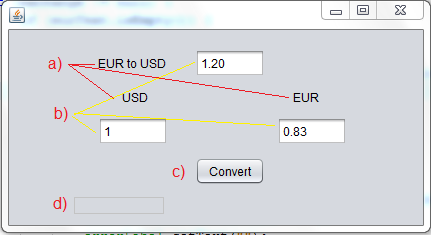
\includegraphics[width=.8\linewidth]{img/gui.png}
\caption{Currency converter: a) labels b) textfields c) button d) notification label}
\label{fig:gui}
\end{figure}

\end{document}